%!TEX root = ../scivis_lbaakman_bvanloon.tex
In \cref{fig:colormapping:colormaps} a visualization from simulation snapshot is shown using all the different colormaps available in the application. Looking at the difference between colormaps we can note a few things. Looking at the visualization that uses the rainbow colormap (\cref{fig:colormapping:intro:differntColorMaps:rainbow}) we see that the maxima are very prominent and that there is a clear distinction between the blue, green, and green areas but no clear transition between those areas. This conforms the disadvantages as discussed in \cref{ssub:rainbow_colormap}.  When we look at the visualization using the zebra colormap in \cref{fig:colormapping:intro:differntColorMaps:zebra} we see that this colormap indeed shows the difference between areas with high variation and low variation. 

\begin{figure}[htb]
	\centering
	\begin{subfigure}{0.35\textwidth}
		\centering
		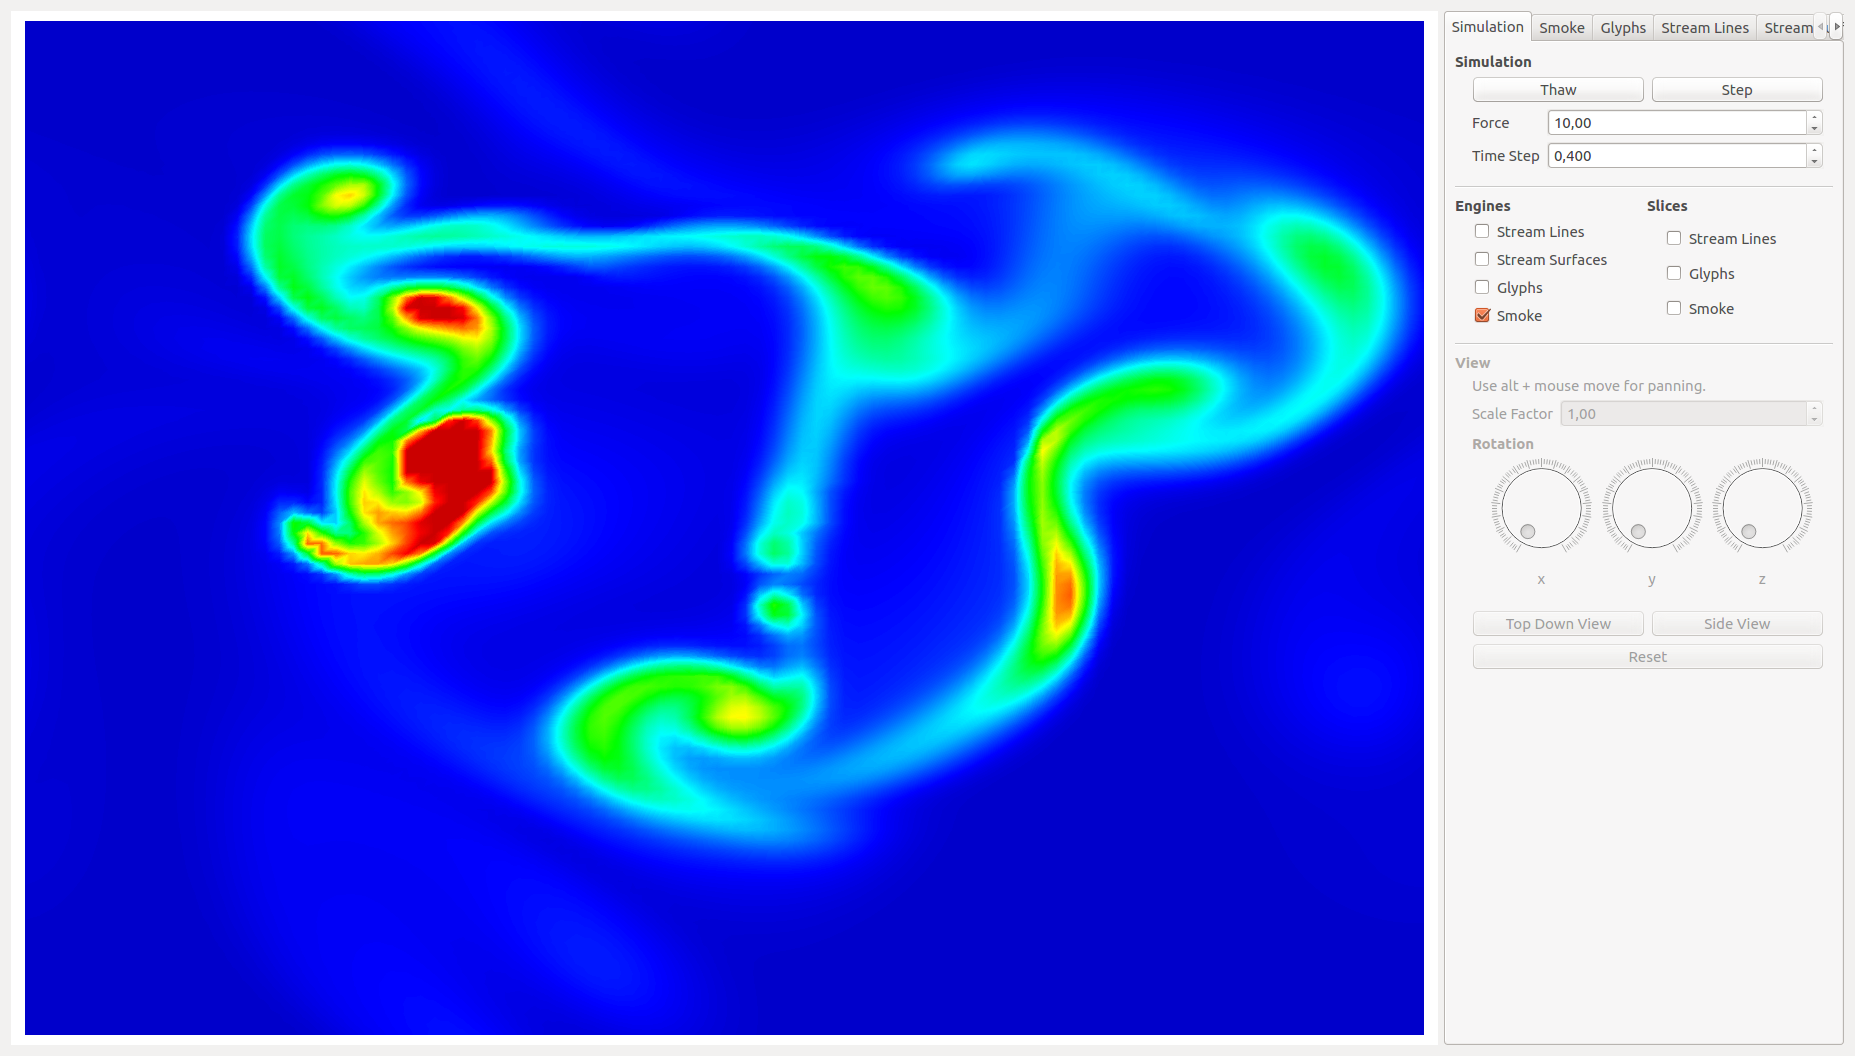
\includegraphics[width=0.9\textwidth, trim={35px 30px 430px 30px}, clip]{colormapping/img/rainbow}
		\begin{tikzpicture}
		    \node[anchor=south west,inner sep=0] (image) at (0,0) {
\includegraphics[rotate=90,width=0.03\textwidth,height=95px,keepaspectratio=false,frame]{colormapping/img/colormap_legends/rainbowcolormap}};
		\end{tikzpicture}
		\caption{Rainbow}
		\label{fig:colormapping:intro:differntColorMaps:rainbow}
	\end{subfigure}
	\hspace{30px}
	\begin{subfigure}{0.35\textwidth}
		\centering
		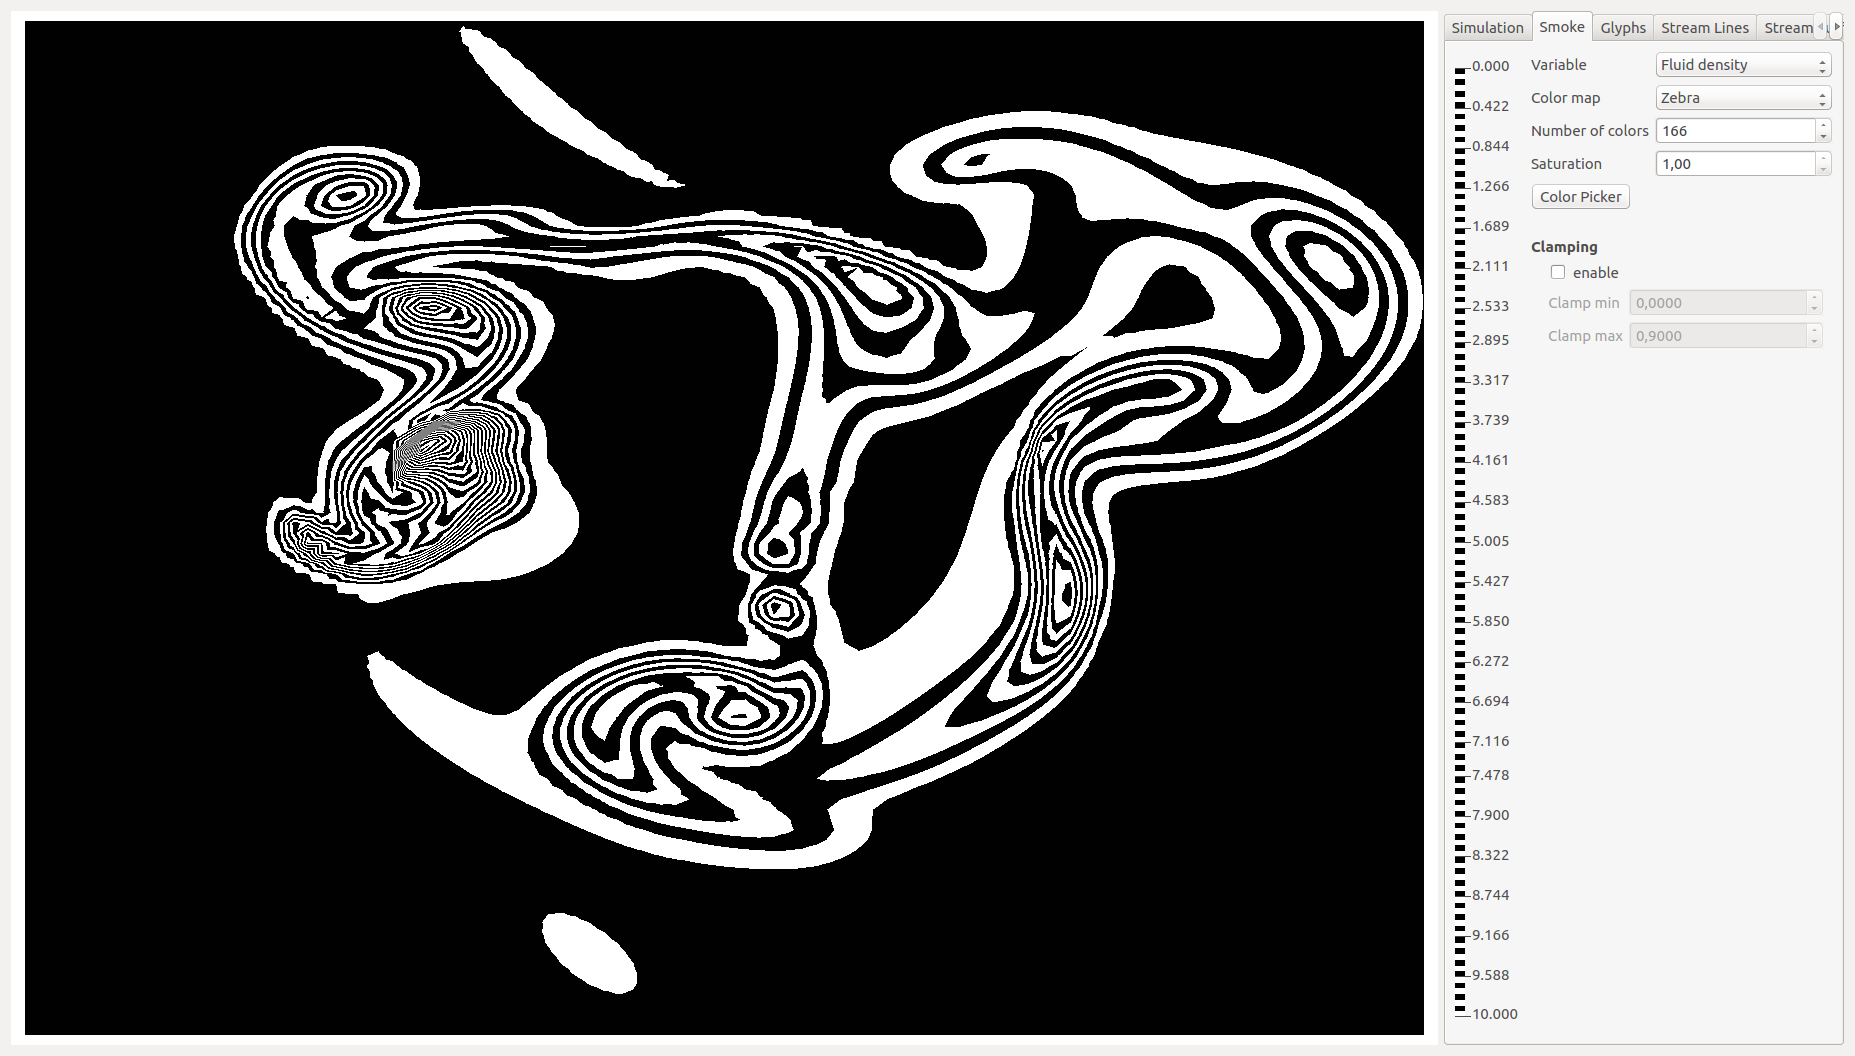
\includegraphics[width=0.9\textwidth, trim={35px 30px 430px 30px}, clip]{colormapping/img/zebra_166}
		\begin{tikzpicture}
		    \node[anchor=south west,inner sep=0] (image) at (0,0) {
\includegraphics[rotate=90,width=0.03\textwidth,height=95px,keepaspectratio=false,frame]{colormapping/img/colormap_legends/zebracolormap}};
		\end{tikzpicture}
		\caption{Zebra}
		\label{fig:colormapping:intro:differntColorMaps:zebra}
	\end{subfigure}
\caption{A visualization of the \emph{Fluid Density} using different colormaps available in the application. All colormaps uses 256 colors except for the zebra colormap which uses 50. All colormaps are fully saturated.}
\end{figure}


Looking at the results when the gray-scale, single hue, heat, and cold colormaps are used (\cref{fig:colormapping:intro:differntColorMaps:grayscale} to \ref{fig:colormapping:intro:differntColorMaps:cold}) we see in all cases a nice transition (and ordering) from areas with low to areas with high values. Also note the added benefit of the maps containing hues compared to the gray-scale colormap; especially in the areas containing low values a bit more variation is visible.

\begin{figure}[htb]
\centering
\ContinuedFloat
	\begin{subfigure}{0.35\textwidth}
		\centering
		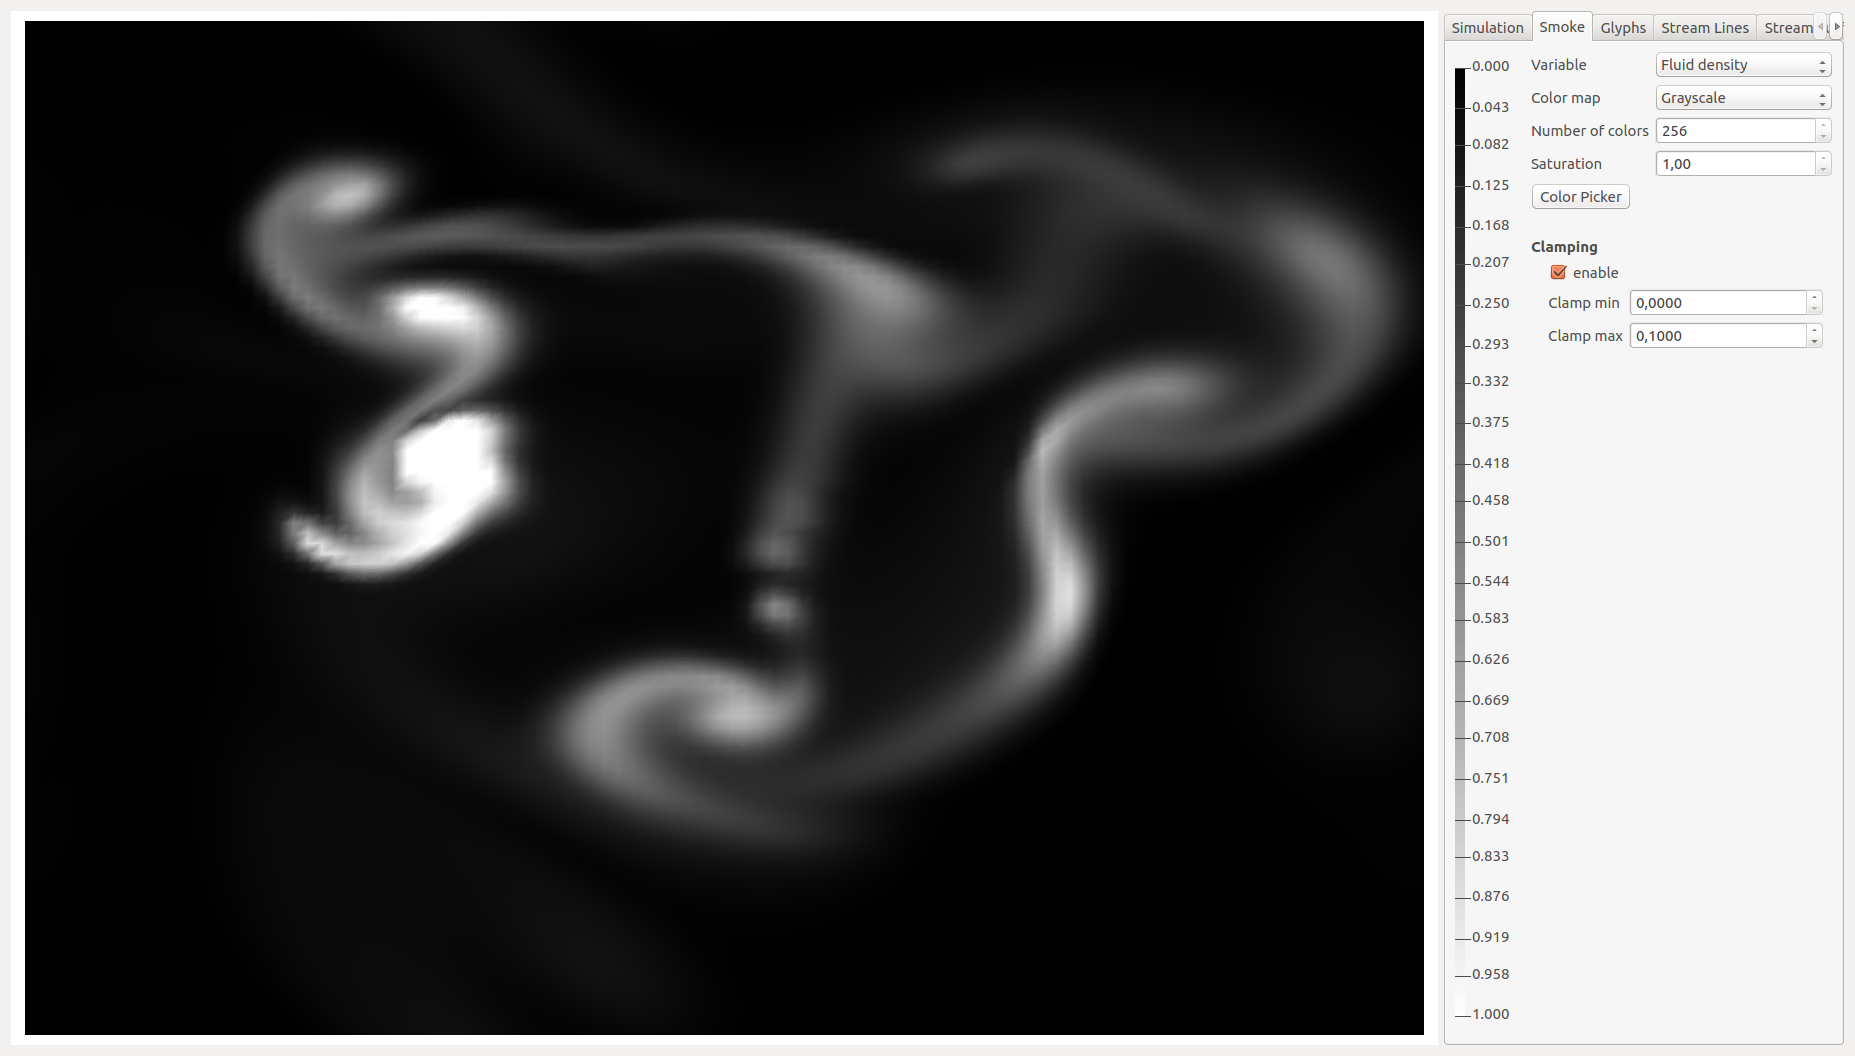
\includegraphics[width=0.9\textwidth, trim={35px 30px 430px 30px}, clip]{colormapping/img/grayscale}
		\begin{tikzpicture}
		    \node[anchor=south west,inner sep=0] (image) at (0,0) {
\includegraphics[rotate=90,width=0.03\textwidth,height=95px,keepaspectratio=false,frame]{colormapping/img/colormap_legends/grayscalecolormap}};
		\end{tikzpicture}
		\caption{
		Gray-scale.
		}
		\label{fig:colormapping:intro:differntColorMaps:grayscale}
	\end{subfigure}
		\hspace{30px}
	\begin{subfigure}{0.35\textwidth}
		\centering
		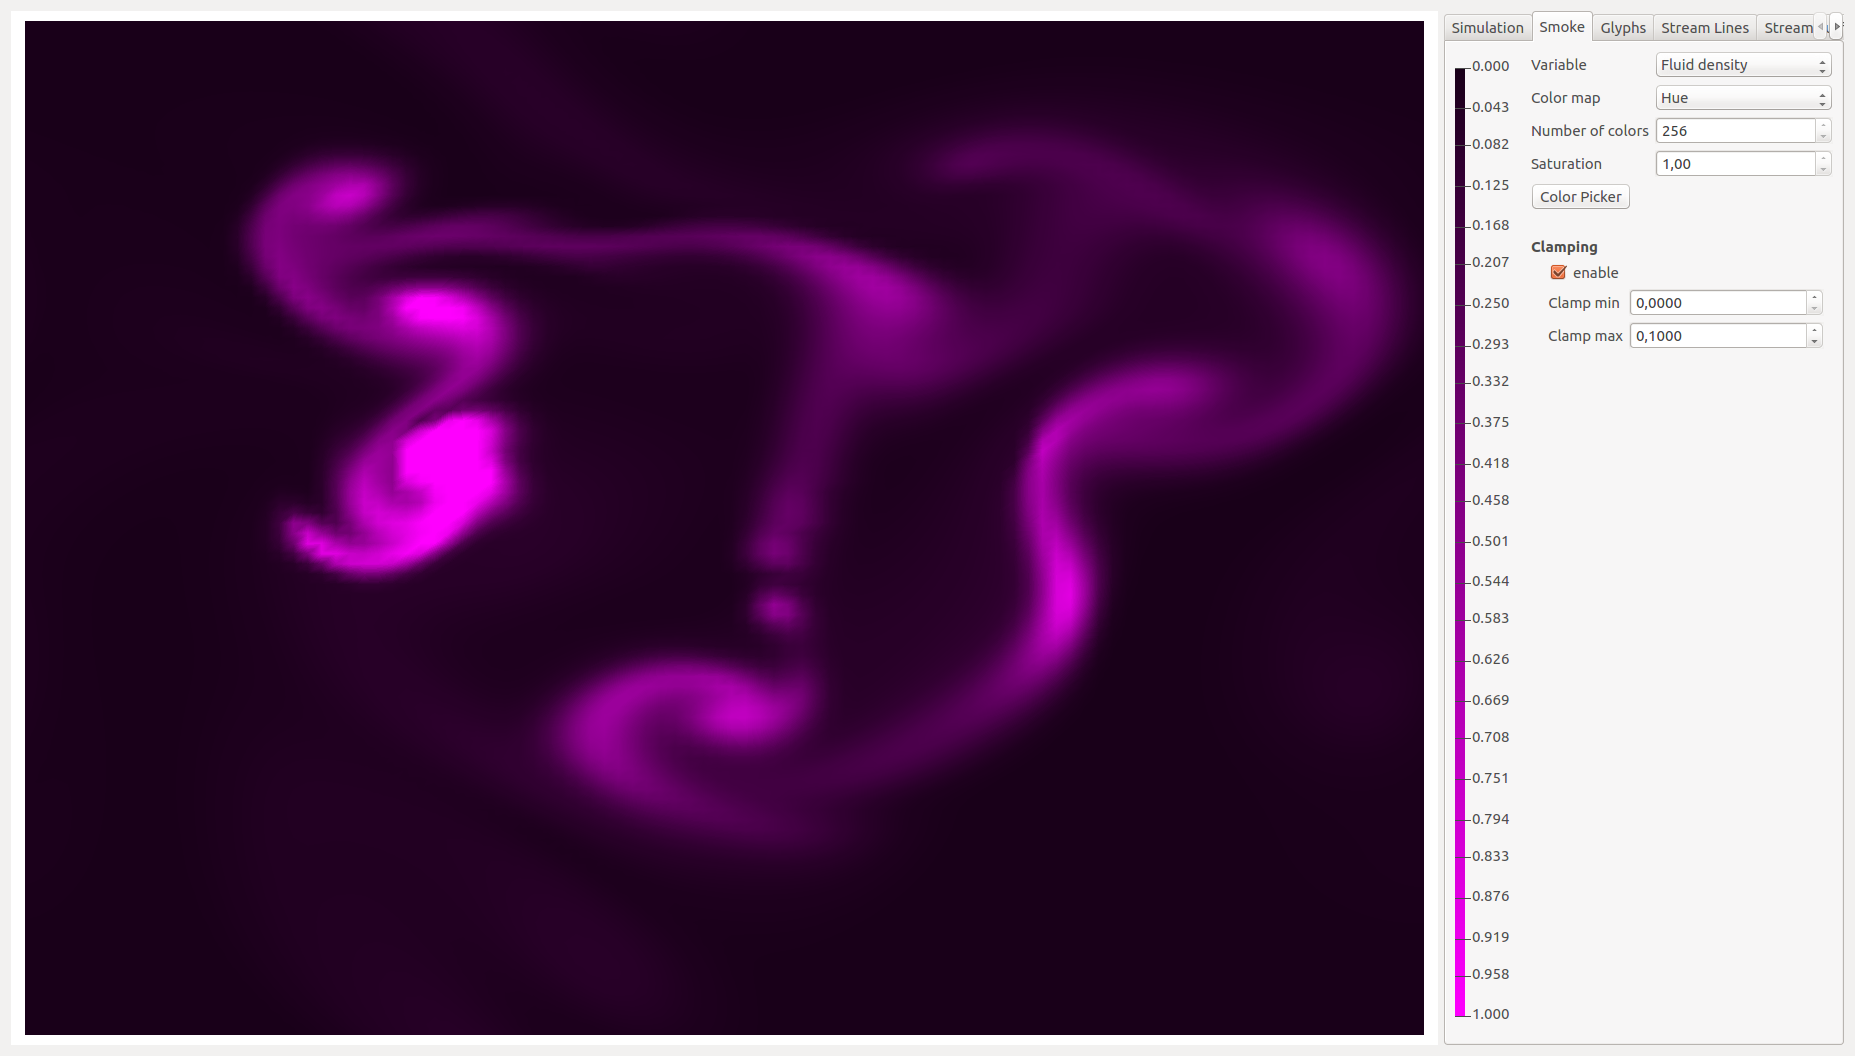
\includegraphics[width=0.9\textwidth, trim={35px 30px 430px 30px}, clip]{colormapping/img/hue}
		\begin{tikzpicture}
		    \node[anchor=south west,inner sep=0] (image) at (0,0) {
\includegraphics[rotate=90,width=0.03\textwidth,height=95px,keepaspectratio=false,frame]{colormapping/img/colormap_legends/huecolormap}};
		\end{tikzpicture}
		\caption{
		Hue (Pink)
		}
		\label{fig:colormapping:intro:differntColorMaps:hue}
	\end{subfigure}
	\begin{subfigure}{0.35\textwidth}
		\centering
		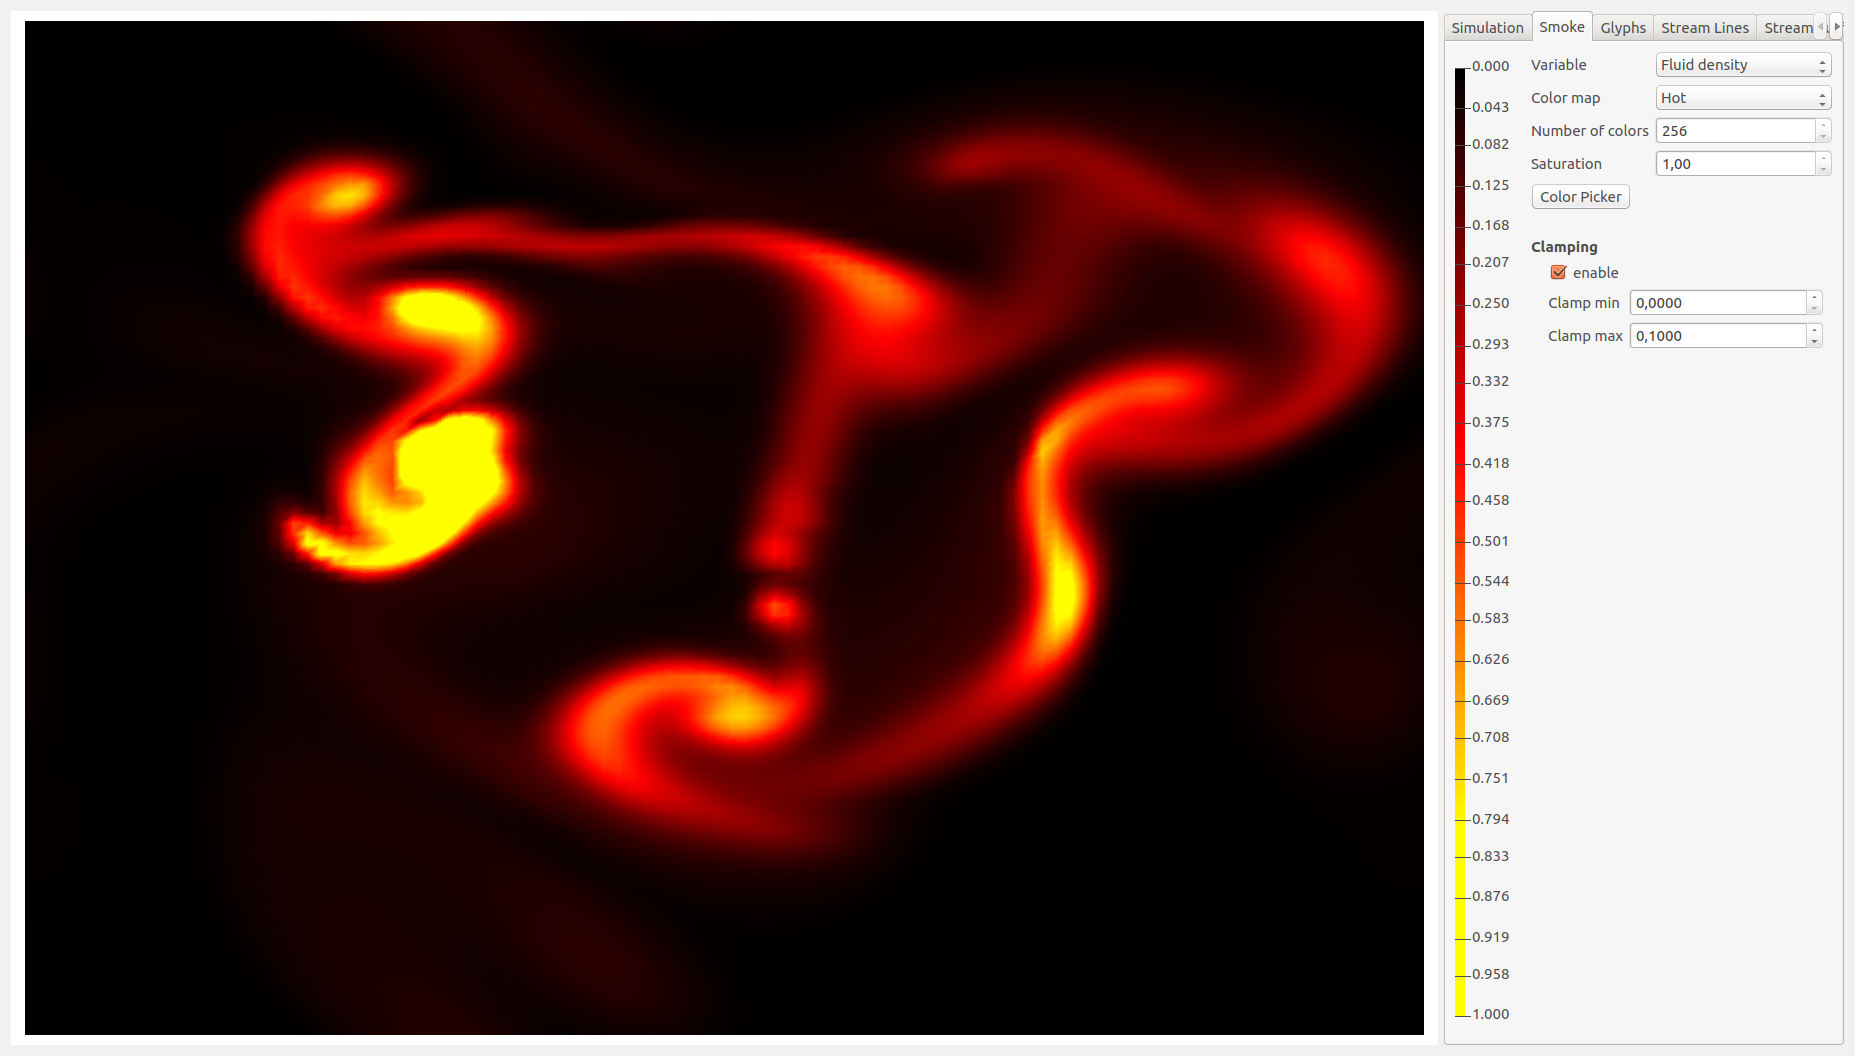
\includegraphics[width=0.9\textwidth, trim={35px 30px 430px 30px}, clip]{colormapping/img/heat}
		\begin{tikzpicture}
		    \node[anchor=south west,inner sep=0] (image) at (0,0) {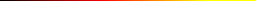
\includegraphics[rotate=90,width=0.03\textwidth,height=95px,keepaspectratio=false,frame]{colormapping/img/colormap_legends/heatcolormap}};
		\end{tikzpicture}
		\caption{
		Heat
		}
		\label{fig:colormapping:intro:differntColorMaps:heat}
	\end{subfigure}
		\hspace{30px}
	\begin{subfigure}{0.35\textwidth}
		\centering
		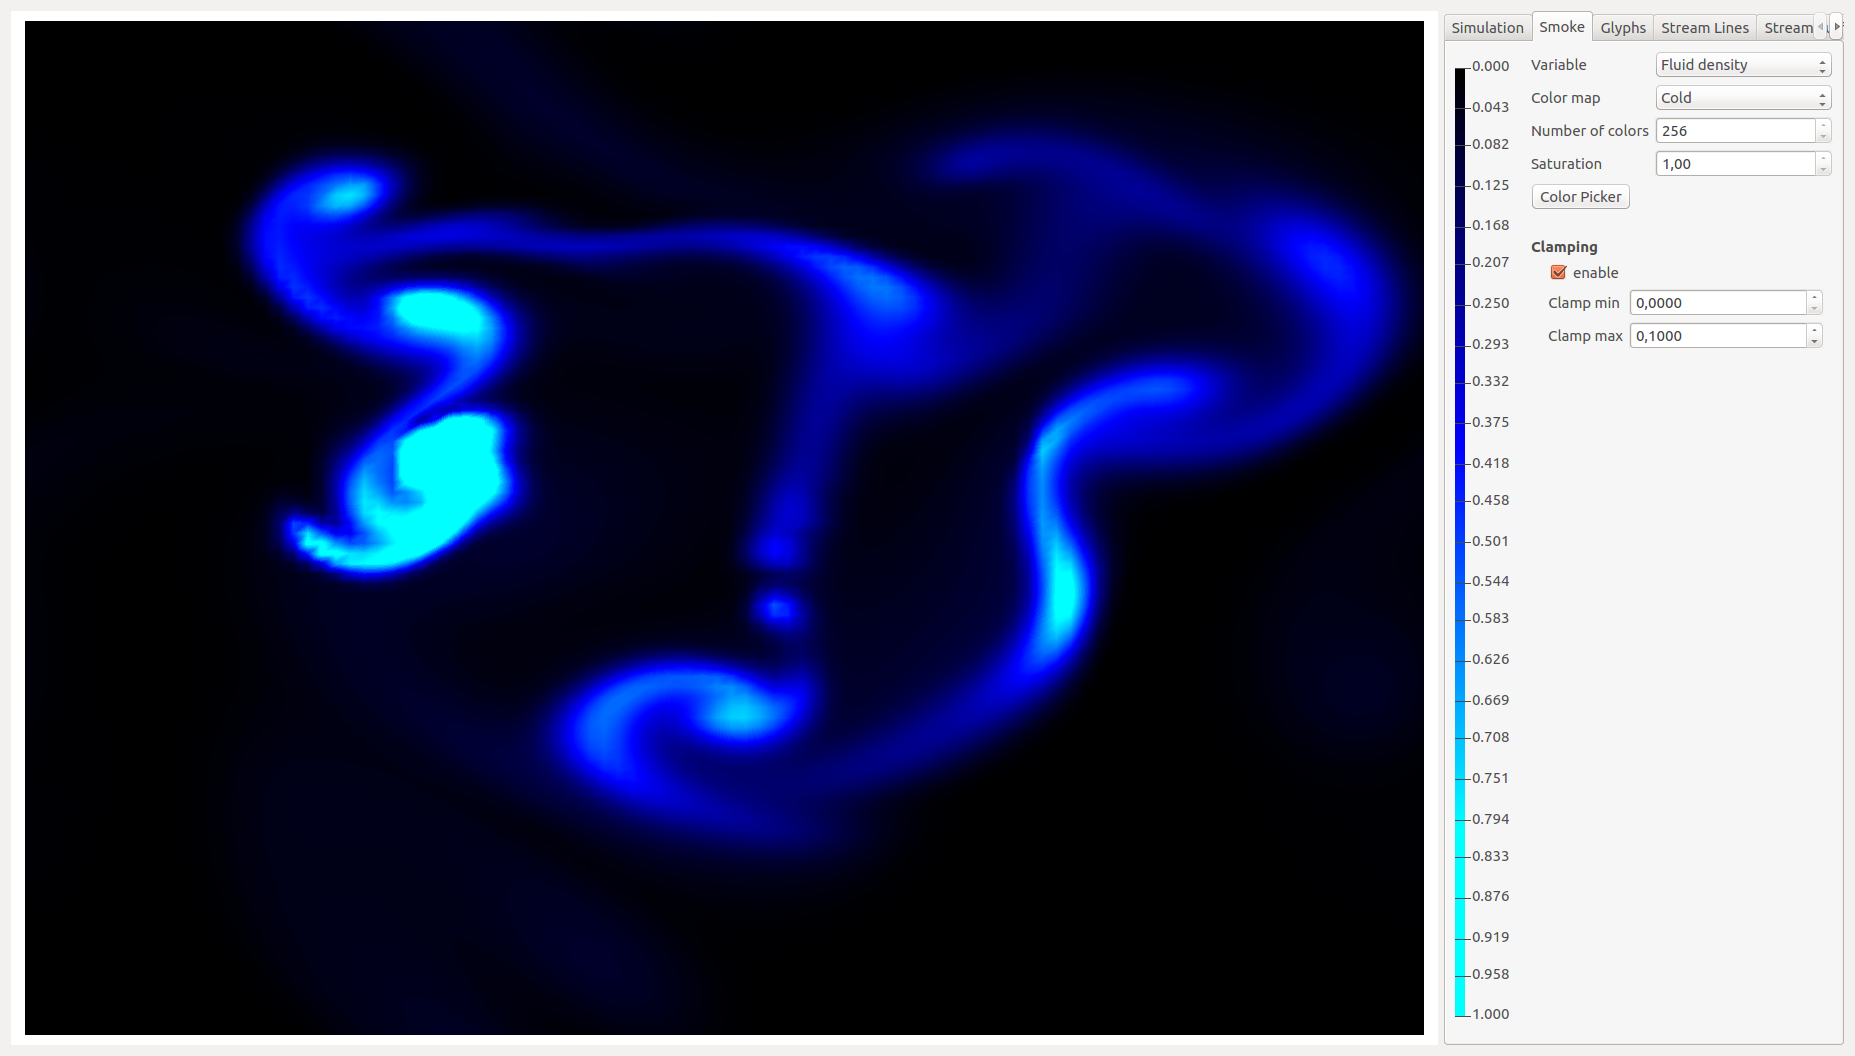
\includegraphics[width=0.9\textwidth, trim={35px 30px 430px 30px}, clip]{colormapping/img/cold}
				\begin{tikzpicture}
		    \node[anchor=south west,inner sep=0] (image) at (0,0) {
\includegraphics[rotate=90,width=0.03\textwidth,height=95px,keepaspectratio=false,frame]{colormapping/img/colormap_legends/coldcolormap}};
		\end{tikzpicture}
		\caption{
		Cold
		}
		\label{fig:colormapping:intro:differntColorMaps:cold}
	\end{subfigure}
\caption{Continued}
\end{figure}
When looking at the results for the isoluminant blue-red colormap in \cref{fig:colormapping:intro:differntColorMaps:twocolor} we see that the colormap does not offer as much details as the other colormaps. This confirms that these colormaps are not well suited for 2D visualizations. 

Last we look at the visualization using the  diverging colormap in \cref{fig:colormapping:intro:differntColorMaps:diverging}. We can see the same distinct areas as with the rainbow colormap, showing clear difference between high and low areas. Compared to the rainbow colormap, there are two distinct differences. First the maxima do not draw as much attention as in the rainbow colormap, furthermore we can see a more natural transition from low to high values making this colormap more suitable.


\begin{figure}[htb]
\ContinuedFloat	
\centering
	\begin{subfigure}{0.35\textwidth}
		\centering
		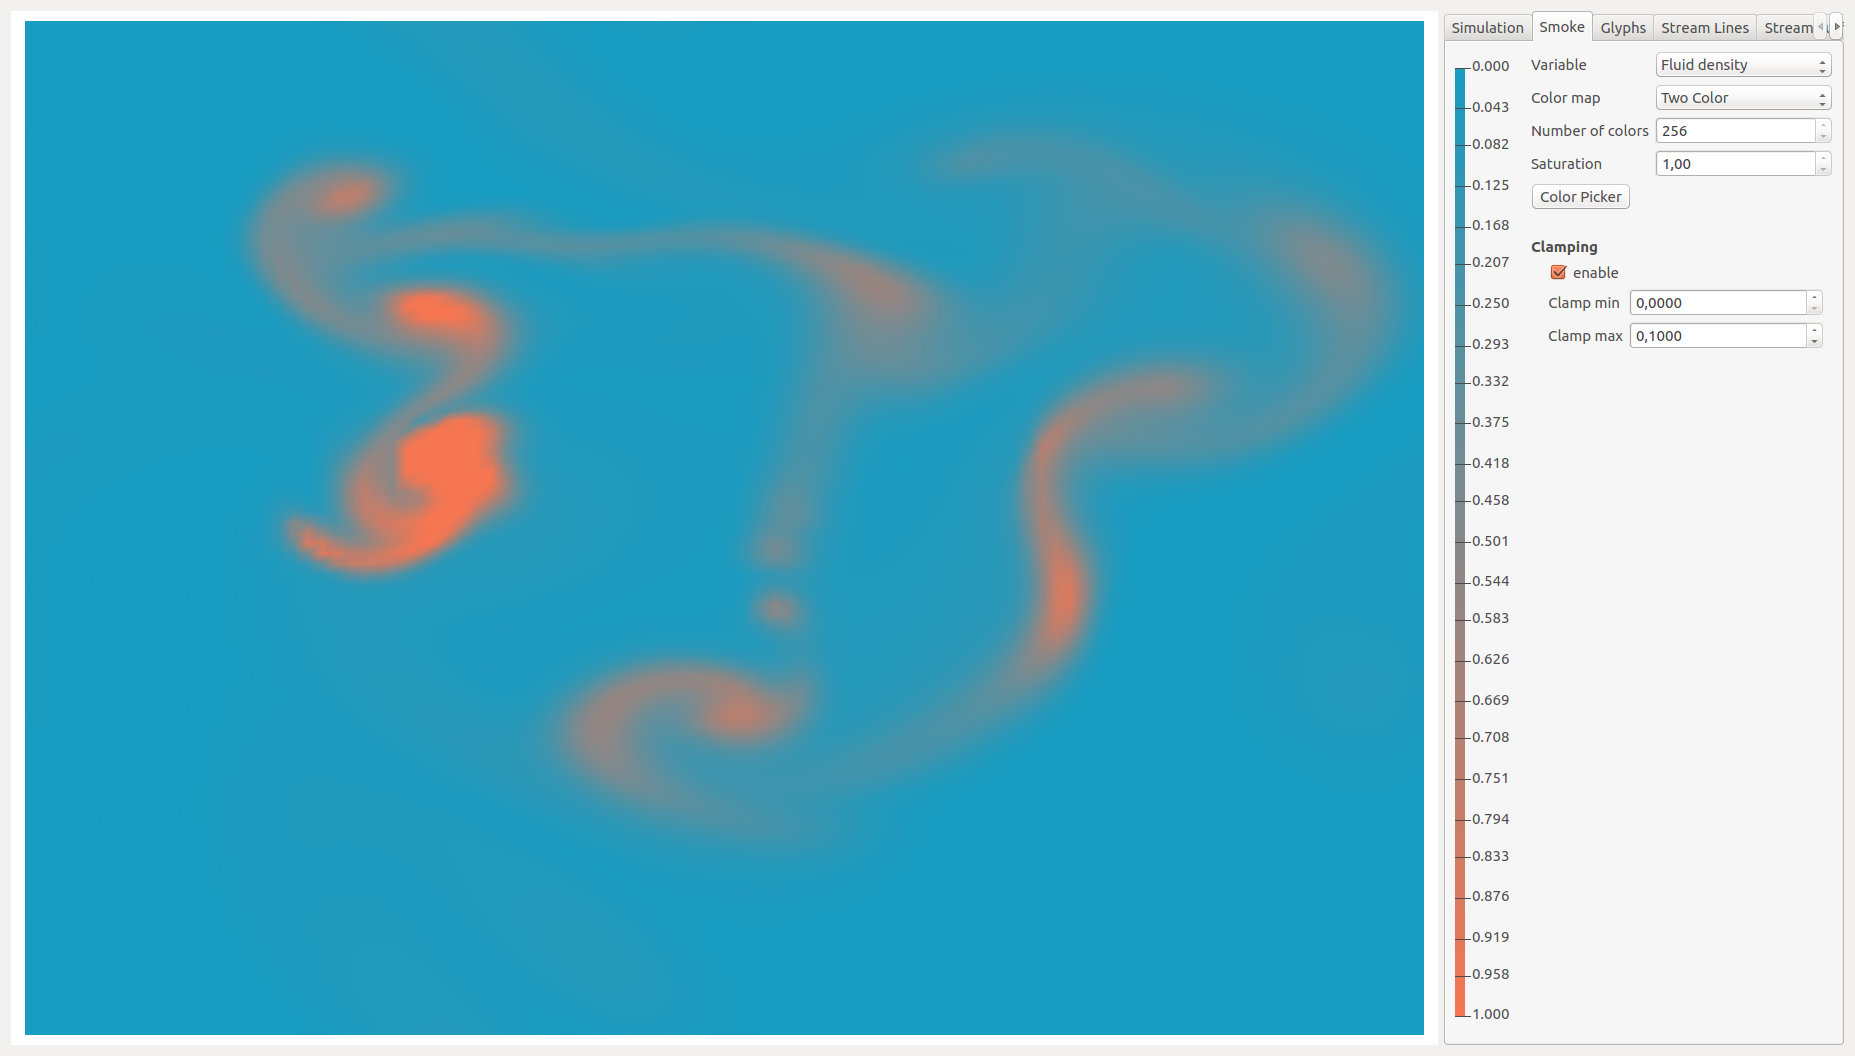
\includegraphics[width=0.9\textwidth, trim={35px 30px 430px 30px}, clip]{colormapping/img/twocolors}
		\begin{tikzpicture}
		    \node[anchor=south west,inner sep=0] (image) at (0,0) {
\includegraphics[rotate=90,width=0.03\textwidth,height=95px,keepaspectratio=false,frame]{colormapping/img/colormap_legends/twocolorscolormap}};
		\end{tikzpicture}
		\caption{
		Isoluminant Blue-Red
		}
		\label{fig:colormapping:intro:differntColorMaps:twocolor}
	\end{subfigure}	
	\hspace{30px}
	\begin{subfigure}{0.35\textwidth}
		\centering
		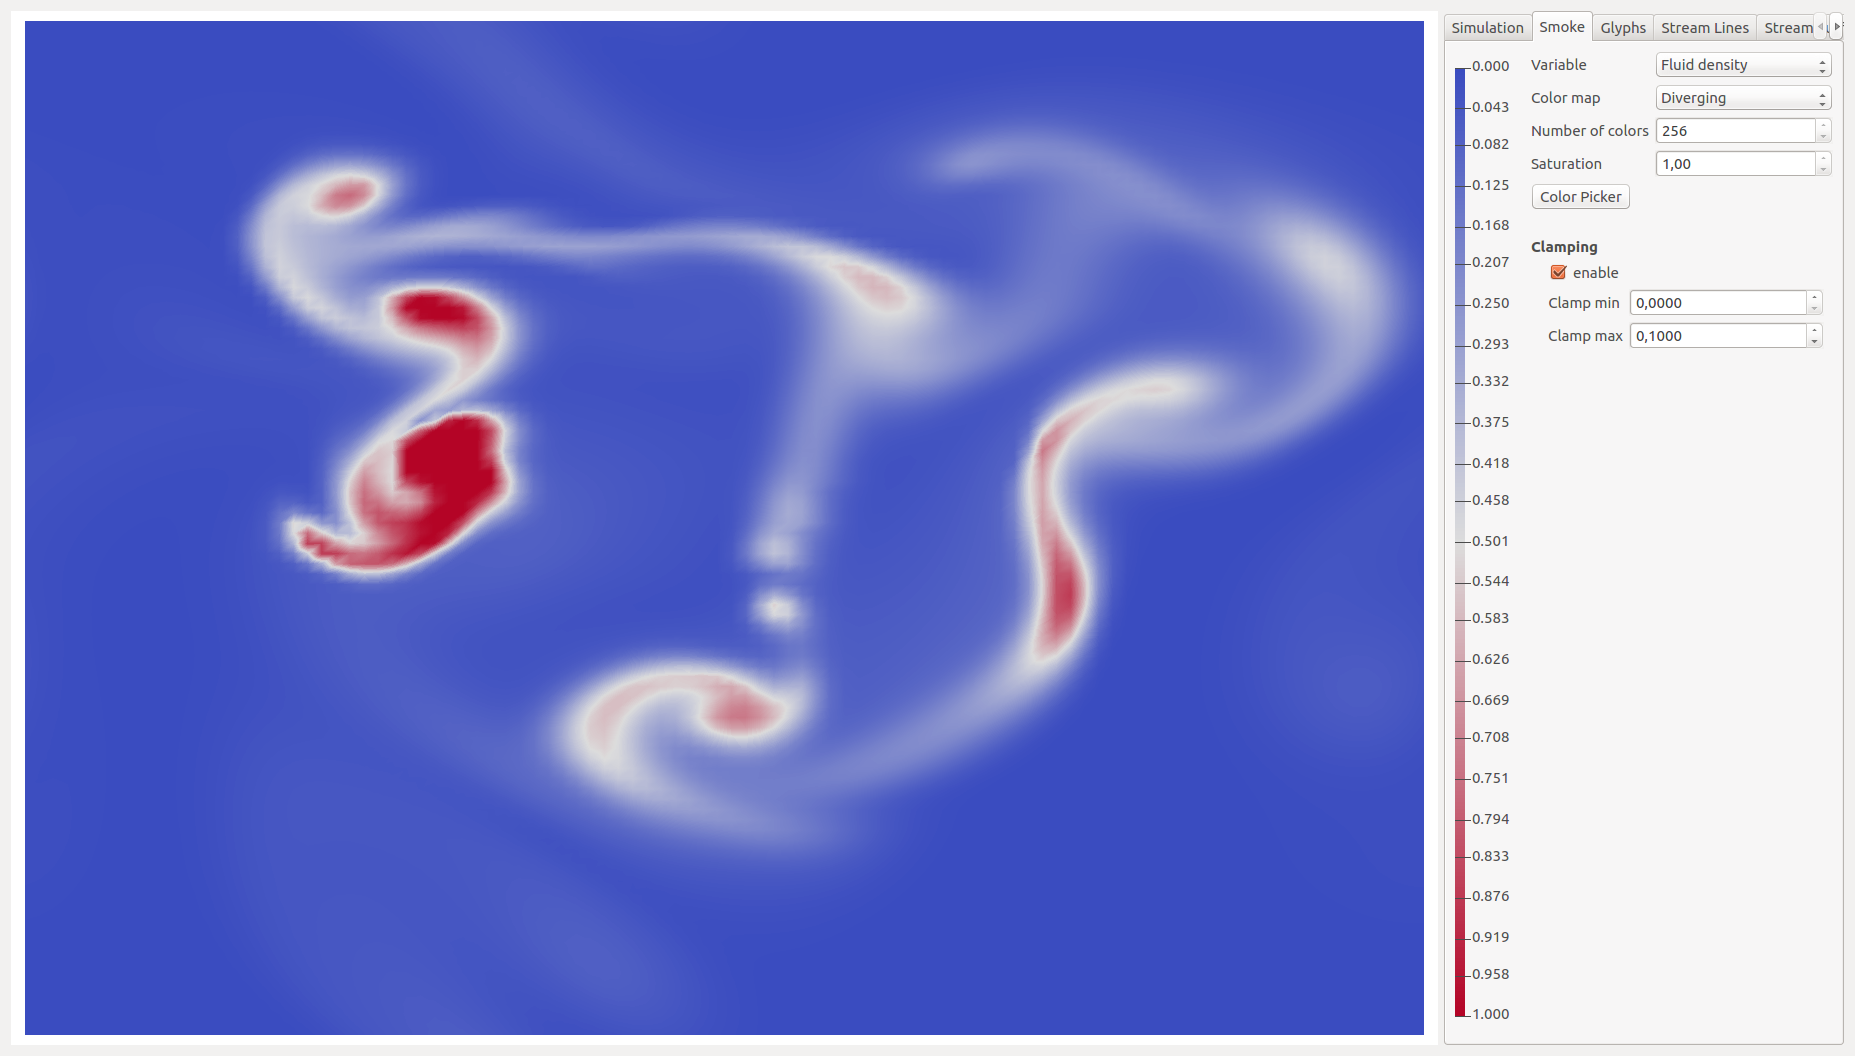
\includegraphics[width=0.9\textwidth, trim={35px 30px 430px 30px}, clip]{colormapping/img/diverging}
		\begin{tikzpicture}
		    \node[anchor=south west,inner sep=0] (image) at (0,0) {
\includegraphics[rotate=90,width=0.03\textwidth,height=95px,keepaspectratio=false,frame]{colormapping/img/colormap_legends/divergingcolormap}};
		\end{tikzpicture}
		\caption{
		Diverging
		}
		\label{fig:colormapping:intro:differntColorMaps:diverging}
	\end{subfigure}				

	\caption{Continued.}
	\label{fig:colormapping:colormaps}
\end{figure}